\chapter{Potential Leakage Sources}

In this chapter, we discuss the potential leakage sources in the environment we have set up in \Cref{Chp: Experiment Setup}. 

%\section{A review of review: what could be leaked?} \label{Sec: A Review of Review}
%What is ``Information''

%The first and fundamental question that must be clarified in this project is: what is ``information''?
%
%If we review those attacks described in \Cref{Chp: Literature Review}:
%
%\begin{itemize}
%	\item In literatures about the flaws in implementations of algorithms and protocols, ``information'' is the plaintext, usually represented as a numerical value, such as \cite{802154sec} \cite{rfc7457} \cite{CompressionRatioAttack} \cite{PaddingOracle}. Or it could be the secret key materials in many cryptographic side channel attack literatures, such as \cite{DPA}.
%	\item In Traffic Analysis Attacks against web applications, ``informaiton'' is the user input, such as \cite{PinpointWeb} \cite{SearchAttack}, or the content of websites such as \cite{WebSideChannel}.
%	\item When we talk about website fingerprinting such as \cite{WebsiteFingerprint} \cite{Peekaboo} and \cite{PClassifier}, ``information'' is the identity of websites. 
%	\item The category only gets even more messy and trivial when we look at other Traffic Analysis Attacks, such as the spoken language and phrases in \cite{VoIPLanguage} and \cite{VoIPPhrases}, user event and OS of Apple product in \cite{AppleMessage} or even the ambient change and motion event in \cite{Video}.
%\end{itemize}
%
%``Information'' is always a relative concept to ``application'', and so is ``leakage''. 

\section{Objects} \label{Sec: Objects}

Without loss of generality, in this report, we are interested on leakages with respect to the following objects:

\begin{description}[style=nextline]
	\item[Content and Size of Application Data]
	The implication of Application Data varies in each application.
	
	\item[Cryptographic Key]
	This represents the corresponding key materials in the security measure.
	
	\item[Network Topology]
	This implies how Sensor Nodes are connected to each other.
	
	%\item[Application Specific Feature]
\end{description}

In this chapter we give a theoretical general analysis of the information leakage from the Traffic Analysis aspect. The inspection of protocol and implementation flaws are included in later chapters.

Notice that Traffic Analysis is highly application specific. In this report, we discuss only the applications described in \Cref{Sec: Applications}. 

\section{Observables} \label{Sec: Observables}

As we have explained in \Cref{Chp: Experiment Setup}, we assumed the adversary has full access to all traffic being transmitted in the WSN. 

\begin{figure*}[h!]
	\center
	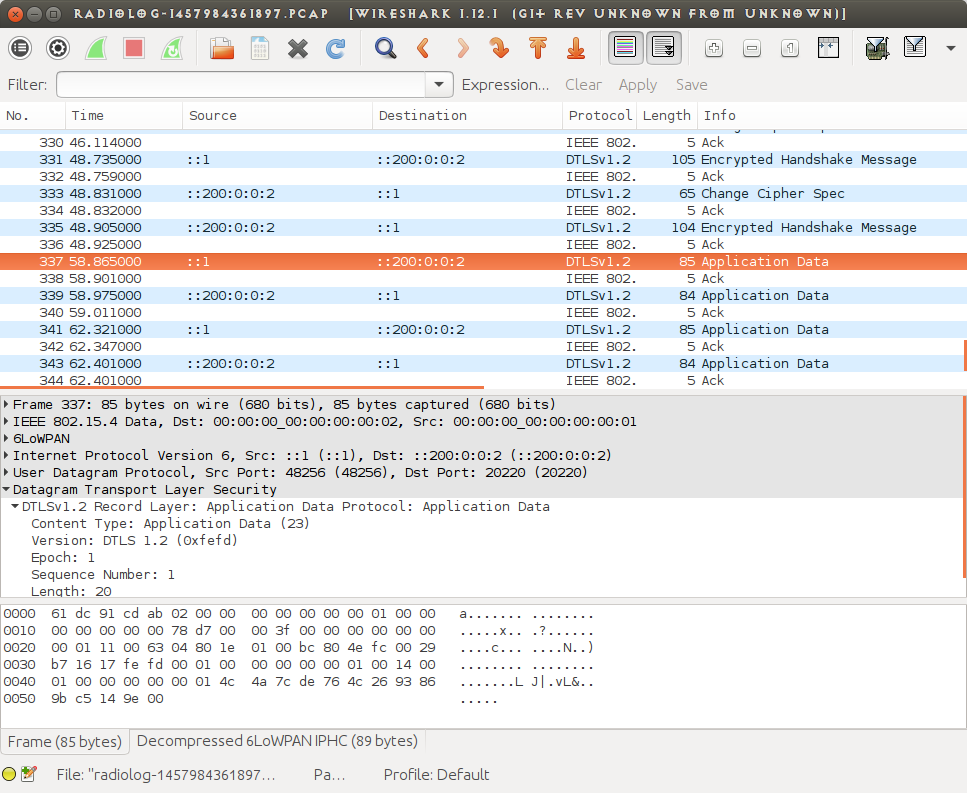
\includegraphics[width=0.9\textwidth]{fig/udpexample.png}
	\caption{An Example of Captured Traffic}
	\label{Fig: An Example of Captured Traffic}
\end{figure*}

\Cref{Fig: An Example of Captured Traffic} is a screenshot of packets in an experiment, analysed by Wireshark\cite{Wireshark}. In this research, we assume the value of ciphertext is independent to the plaintext and key. The following side channel information are available in the captured traffic:

\begin{itemize}
	\item Unencrypted headers
	\item Timing
	\item Length
\end{itemize}

The timing and length information are always available in the captured traffic. The unencrypted headers depend on the security measure adopted, which we explain in later sections.

Practically, the Receive Signal Strength Indicator, RSSI, should also be considered visible to the adversary. RSSI represents the RF signal strength. By measuring the RSSI of frames sent from a specific source MAC address,  it is possible to reveal the geographical information of a specific Sensor Node. However we do not consider RSSI in this report as its physical character is beyond the scope of this project. Instead, we assume the adversary has prior knowledge of all geographic information of Sensor Nodes in the WSN.

%\subsubsection{noncoresec} \label{Subsubsec: noncoresec header}
%
%As explained in \Cref{Subsec: 802.15.4 Security Implementation in Contiki}, noncoresec is the 802.15.4 Security implementation on Contiki. When noncoresec is enabled, all captured frames are in the form we explained in \Cref{Subsec: 802.15.4 MAC} and \Cref{Subsec: 802154 Sec}. The 802.15.4 MAC Header is the only unencrypted part of a packet.
%
%We stated in \Cref{Subsec: noncoresec in experiment} that we always use the highest Security Level of 802.15.4 Security; therefore:
%\begin{itemize}
%	\item MAC Payload is always authenticated and encrypted in AES-128 with CCM* mode.
%	\item Security Level is constantly 0x7.
%	\item Key Strategy is constantly 0x0 as noncoresec does not implement any key management.
%\end{itemize}
%
%As a result of MAC Payload being authenticated and encrypted, 
%\begin{itemize}
%	\item The adversary cannot join the 6LoWPAN network as we have explained in \Cref{Subsec: noncoresec in experiment}.
%	\item The adversary cannot directly distinguish an IPv6 packet and an ICMPv6 packet by the contents in MAC Payload as it is encrypted. 
%\end{itemize}
%
%%In our experiments, the application data is effectively sent in IPv6 packets. ICMPv6 packets on the other hand are mostly RPL messages.
%
%\subsubsection{DTLS} \label{Subsubsec: DTLS header}
%
%As explained in \Cref{Chp: Building Blocks}, when DTLS is used, the explicit observables are: 
%
%\begin{itemize}
%	\item 802.15.4 MAC Header as explained in \Cref{Subsec: 802.15.4 MAC}.
%	
%	\item Compressed IPv6 Header as explained in \Cref{Subsec: 6LoWPAN Adaptation Sub Layer}, \Cref{Subsec: IPv6 Data Packets} and \Cref{Subsec: ICMPv6}.
%	
%	\item UDP Header as explained in \Cref{Subsec: UDP}.
%	
%	\item DTLS Header as explained in \Cref{Subsec: DTLS}.
%\end{itemize}
%
%Since DTLS is built on Application Layer, therefore it does not impose any setting to the lower layer headers. 

\section{Packet Traces} \label{Subsec: Traces}

In this section, we discuss some features of packet traces in WSN applications.

%Before discussing the ``traces'' in WSN applications, as a comparison, we review the different definition of ``traces'' in the literatures we reviewed in \Cref{Chp: Literature Review}:
%
%\begin{itemize}
%	\item In literatures about Traffic Analysis Attacks against web applications\cite{WebSideChannel}\cite{PinpointWeb}\cite{SearchAttack}, a ``trace'' refers to the continuous\footnote{We would argue that the term ``continuous'' is ambiguous; nevertheless it is the best definition we can thought of.} packets triggered by an user input.
%	\item In Website Fingerprinting literatures\cite{WebsiteFingerprint} \cite{HClassifier} \cite{PClassifier} \cite{Peekaboo}, a ``trace'' refers to the continuous packets that triggered by a browser requesting a website.
%	\item Other attacks use more specific application dependent definitions of a ``trace''. \cite{VoIPLanguage} and \cite{VoIPPhrases} defined a ``trace'' to be the continuous packets during a VoIP conversation. \cite{Video} defines it to be the continuous packets during a video conversation. \cite{AppleMessage} does not even use the term ``trace'' at all\footnote{Actually it did used once as a verb equivalent to ``track''.} as it only analyses a single packet.
%\end{itemize}
%
%Practically, the ``trace'' of an Internet application can be defined by filtering packets belong to the same TCP connection,or UDP packets with the same entities\footnote{An entity is the combination of an IP address and a port}. However, we cannot apply the same method on many WSN applications due to the change of protocol suite and application nature. For example, TCP is not used as explained in \Cref{Chp: Building Blocks} and communication are mostly done with ephemeral ports. Further more, the WSN applications perform Machine To Machine, M2M, communication which has much less external intervention, makes it harder to group packets into ``traces''.

WSN application designs tend to be simple and stateless by its nature of constrained resources and underlining protocol suite. In another word, data transmission is minimised for efficiency and data exchanging need be idempotent to maintain robustness. From this aspect, we argue that the simple applications we developed in \Cref{Sec: Applications} have captured these most significant characteristics of WSN applications.

In this report, we define a generic model for the data exchanging process in the WSN applications.

\begin{definition} \label{Def: Session}
A Session is defined as a series of events where a Sensor Node reports application data to a Manager. A Session includes an optional Request sent from Manager to Sensor Node, and a Response containing the requested data sent from Sensor Node to Manager.
\end{definition}

\begin{definition} \label{Def: Trace}
A trace is defined as all captured packets within one Session.
\end{definition}

Although not necessary under \Cref{Def: Session}, in most of our applications, there are typically one or two packets in a trace. The first one corresponds to Request and the second corresponds to Response. In some applications such as broadcast keyllsec in \Cref{Sec: Applications} or a CoAP application using OBSERVE option in \Cref{Subsec: CoAP}, there might be only one Response packet in a trace without a Request. In real world applications there might even be a Request without a Response, e.g. a command to control a light bulb. However, in this report, we define there is at least one packet corresponds to Response. We further assume the adversary is aware of the application running on the Sensor Nodes. Consequently, the adversary in our setting is able to distinguish a Request and a Response, but has no knowledge of the application data being transmitted within them.

We also assume the adversary is capable to distinguish Sessions. Practically, the time interval of packets within the same Session are usually significantly less then the interval between Sessions. \Cref{Fig: Example Traces of keyllsec} shows an example of traces in a unicast keyllsec application instance, with \textcircled{1} being the sender and \textcircled{2} being the receiver. Marked are packets for two continuous Sessions, where No.977 and No.990 is the first Session and No.998 and No.1011 are the second. We can see that the time interval within a Session is about 150ms which is significantly less than the 15s interval between Sessions.

\begin{figure*}[h!]
	\center
	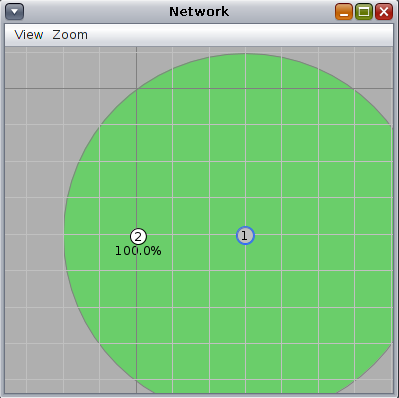
\includegraphics[width=0.5\textwidth]{fig/unicast_keyllsec.png}
	\\
	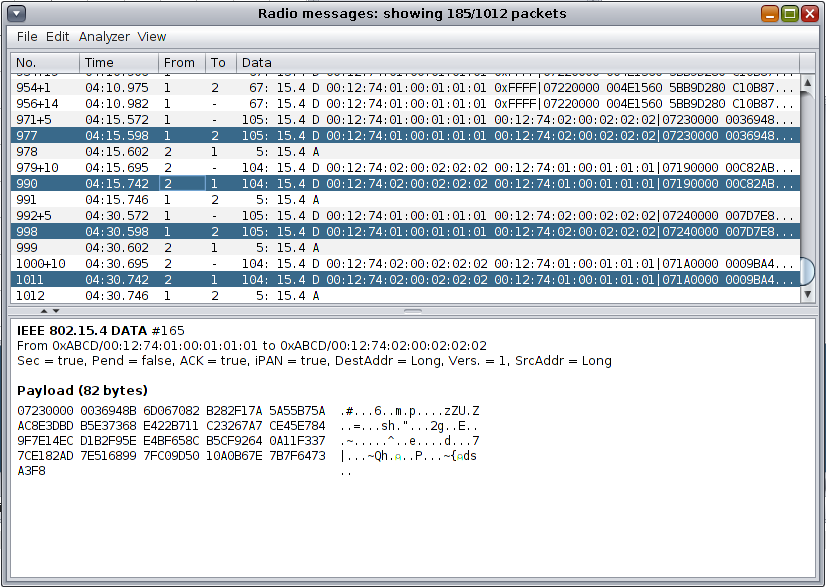
\includegraphics[width=0.9\textwidth]{fig/trace_keyllsec.png}
	\caption{Example Traces of keyllsec}
	\label{Fig: Example Traces of keyllsec}
\end{figure*}

In this project, we consider only information leakage within one Session. It is arguably that there is potential leakage when jointly analyse traces from different Sessions, e.g. the frequency of Requests can ``leak'' itself. However, we omit such leakage for generality as exploiting them requires further assumptions to the higher level application. Each Session in this report is also considered to be independent based on that fact that each execution of our code is independent to its last execution.

%Further more, in our applications the content of Request is a constant 3 bytes ASCII string ``GET''. We assume this known by the adversary. We make this assumption to focus on the leakage of the Application Data in Responses. 

\section{Theoretical Analysis}

In this section we provide a theoretical analysis over all observables we explained in \Cref{Sec: Observables}. It is done in two approaches:

\begin{enumerate}
	\item Cross reference the intersection of the observables we explained in \Cref{Sec: Observables} with the known exploitable side channel information we introduced in \Cref{Sec: Traffic Analysis Attacks}
	\item Semantically analyse the observables. 
\end{enumerate}

%We discuss only the leakage over the attributes we specified in \Cref{Sec: A Review of Review}.

For some of the observables, we claim:

\begin{theorem} \label{Te: IR}
Under the leakage definitions of Mutual Information and g-leakage in \Cref{Subsec: Information Theory}, if an observable $Y$ is independent to a secret $X$, then there is $0$ leakage of $X$ over $Y$.
\end{theorem}

\Cref{Te: IR} intuitively holds. A formal proof is given in \Cref{Prf: IR}.

\begin{corollary} \label{Cor: Constant Leakage}
	An observable $Y$ with a constant value has no leakage under the leakage definitions of  Mutual Information and g-leakage in \Cref{Subsec: Information Theory}.
\end{corollary}

\begin{proof}
	This directly followed by the fact that a constant $y \in Y$ with $P(y) = 1$ is independent to the secret $X$.
\end{proof}

\subsection{Cross Reference of Observables with Known Attacks} \label{Subsec: Cross Reference}

Despite the differences in the nature applications, we discuss the applicability of the packet features those have been exploited in Traffic Analysis Attacks, as we have summarised in \Cref{Tbl: Classifiers in Traffic Analysis Literatures}.

As a result, we only found four features applicable in our settings:
\begin{itemize}
	\item Packet size
	\item Total bytes
	\item Total Time (only for two packets Session)
	\item Total Per-direction Bandwidth
\end{itemize}

All other features have reduced to a constant or not applicable in our settings. The detailed analysis is described in \Cref{Detail Cross Reference}.

\subsection{Semantic Analysis}

In this section, we provide an analysis over the observables based on their semantics we explained in \Cref{Chp: Building Blocks}.

One exception is the address information. Theoretically speaking, any valid address may be used in any packet and thus could be considered independent to the application. However in practice, different data may use different type of transmission, i.e. unicast, multicast or broadcast; thus the family of address could be a potential leakage source to the Application Data. We provide the analysis within this aspect in later chapters.

Some packets can be observed even if no application is running. These packets, mainly RPL messages, are generated by Contiki kernel to maintain the connectivity of the 6LoWPAN network. Since the existence of these packets is independent to the application running over WSN, we consider them as non leakable due to \Cref{Te: IR}. One exception is the DAO message we explained in \Cref{Subsec: ICMPv6} which could be triggered by the first application packet if the routing is not queried before. In this report, we consider the DAO message independent to the application.

As we have explained in \Cref{Chp: Building Blocks}, the 6LoWPAN protocol suite is constructed layer by layer and each layer is conceptionally transparent to other layers. As a result, most of the headers are in theory independent to the application and thus are non leakable due to \Cref{Te: IR}. For these observables, we expect to see them distributed independently among different applications. Specifically, the choice of cryptographic key is expected to be independent to all contents in the headers.

\subsubsection{Implicit Observables}

The implicit observables are indeed covered by the potential leakage sources we analysed in \Cref{Subsec: Cross Reference}. As a matter of fact, these observables turned out to be the most exploitable features in the literatures we have reviewed in \Cref{Sec: Traffic Analysis Attacks}.

%Linear relationship of length
In our experiments, we noticed that in our security measures, namely noncoresec and DTLS, the underlining cryptographic primitives are both AES-128 with CCM mode where no padding is applied. This effectively indicates that the length of plaintext and ciphertext are expected to have a linear relationship with slope ratio $1$:

\begin{equation} \label{Eq: Linear Length}
	l_{C} = l_{P} + b
\end{equation}

where $l_{C}$ and $l_{P}$ are the length in bytes for packets with and without encryption, and $b$ is a predictable constant induced by security measures such as MIC and change of headers. Practically when the security measure increases the packet length to a value exceeding MTU, the packet will be immediately dropped and cannot be observed by an adversary. However, considering the functionality of WSN, we assume the plaintext is always in a reasonable length that does not result into a ciphertext exceeding MTU.

%Leakage with linear relationship
Modelling the leakage of packet length as a channel $C(l_{C},l_{P})$ as in other Information Theoretic approaches we described in \Cref{Subsec: Information Theory}, we have a deterministic channel such that:
\begin{equation}
	C(l_{P}, l_{C}) = P(l_{P} | l_{C}) = 
	\begin{cases}
		1 &\text{if: } l_{C} = l_{P} + b \\
		0 &\text{otherwise}
	\end{cases}
\end{equation}

and

\begin{equation}
	C^{-1}(l_{C}, l_{P}) = P(l_{C} | l_{P}) = 
	\begin{cases}
		1 &\text{if: } l_{C} = l_{P} + b \\
		0 &\text{otherwise}
	\end{cases}
\end{equation}

So

\begin{equation}
	P(l_{P} , l_{C}) = P(l_{P}) P(l_{C} | l_{P}) =
	\begin{cases}
		P(l_{P}) &\text{if: } l_{C} = l_{P} + b \\
		0 &\text{otherwise}
	\end{cases}
\end{equation}

Therefore\footnote{Information Theory defines $0\log{0} = 0$.},
\begin{equation}
	P(l_{P} , l_{C}) \log{P(l_{P} | l_{C})} = 
	\begin{cases}
		P(l_{P})\log{1} = 0 &\text{if: } l_{C} = l_{P} + b \\
		0 \log{0} = 0 &\text{otherwise}
	\end{cases}
\end{equation}

Hence
\begin{equation}
	H(L_{P} | L_{C}) = - \sum_{l_{C} \in L_{C}} \sum_{l_{P} \in L_{P}}P(l_{P} , l_{C}) \log{P(l_{P} | l_{C})} = - \sum_{l_{C} \in L_{C}} \sum_{l_{P} \in L_{P}} 0 = 0
\end{equation}
where $L_{P}$ and $L_{C}$ are the possible length in bytes of encrypted and unencrypted packets.

In this case, the Mutual Information is:
\begin{equation} \label{Eq: MI in length}
	I(L_{P};L_{C}) = H(L_{P}) - H(L_{P} | L_{C} ) = H(L_{P}) - 0 = H(L_{P})
\end{equation}

For the Capacity, according to \Cref{Eq: MI in length}, $I(L_{P};L_{C})$ has its maximum value when $L_{P}$ is uniformly distributed:
\begin{equation} \label{Eq: Cap in length}
	Capacity = \sup_{\forall L_{P}}{I(L_{P};L_{C})} = \sup_{\forall L_{P}}H(L_{P}) = - \sum_{i = 1}^{|L_{P}|}|L_{P}|^{-1}\log{|L_{P}|^{-1}} = \log{|L_{P}|}
\end{equation}

In another word, \Cref{Eq: MI in length} and \Cref{Eq: Cap in length}  imply that averagely all bits of $l_{P}$ is leaked through $l_{C}$.

For the gain function based leakage\cite{GLeakage}, we realised that it would be hard to quantify the leakage without a specific gain function. Therefore instead, we provide an analysis with min-leakage.

In this case, the Posterior Vulnerability is:
\begin{equation}
	\begin{aligned}
		V(\pi_{L_P}, C^{-1}) 
		&= \sum_{l_{C} \in L_{C}} \max_{l_{P} \in L_{P}} \pi_{L_P}[l_P]C^{-1}[l_P,l_C] \\
		&=  \sum_{l_{C} \in L_{C}} P(l_C) \max_{l_{P} \in L_{P}} P(l_P | l_C) \\
	      &= \sum_{l_{C} \in L_{C}} P(l_C) = 1 \\
	\end{aligned}
\end{equation}

Therefore
\begin{equation}
	\begin{aligned}
		H_{\infty}(\pi_{L_{P}}, C^{-1})
		 &= - \log{V(\pi_{L_{P}}, C^{-1})} = - \log1= 0
	\end{aligned}
\end{equation}

Thus the min-leakage is:
\begin{equation}
	\begin{aligned}
	L(\pi_{L_P}, C^{-1}) 
	 &= H_{\infty}(\pi_{L_P}) - H_{\infty}(\pi_{L_{P}}, C^{-1}) \\
	 &= H_{\infty}(\pi_{L_P}) - 0 \\
	 &= H_{\infty}(\pi_{L_P})
	\end{aligned}
\end{equation}

And finally:
\begin{equation}
	ML(C^{-1}) = \sup_{\pi_{L_P}}{L(\pi_{L_P},C^{-1})} =  \sup_{\pi_{L_P}} H_{\infty}(\pi_{L_P}) = \log{|L_P|}
\end{equation}

This result consists with our intuition and the Capacity in \Cref{Eq: Cap in length} that all bits of $l_P$ are leaked through $l_C$.

\subsubsection{Explicit Observables with noncoresec}

As explained in \Cref{Subsubsec: Explicit noncoresec}, the only explicit observables when using noncoresec is the 802.15.4 MAC Header. 

Referring to \Cref{Subsec: 802.15.4 MAC}, there are four types of MAC Frames. However, both Beacon and Command frame are solely used for connection maintenance and are independent to the application running on Sensor Nodes; therefore we consider them as non leakable sources according to \Cref{Te: IR}.

For the Data frame we explained in \Cref{Subsec: 802.15.4 MAC},
\begin{description}[style=nextline]
	\item[Frame Control]
	Among the flags in Frame Control defined by \cite{802154}, we found only two flags potentially related to upper layer application:
		\begin{description}
			\item[Security Enabled]
			When noncoresec is used, this field is constantly $1$. Due to \Cref{Cor: Constant Leakage}, this is not a potential leakage source.
			\item[ACK Required]
			Since MAC ACK is optional and this field can be set by an upper layer application, we suspect this flag as a potential leakage source.
		\end{description}
	\item[Sequence Number]
	Sequence Number is solely managed by MAC Layer and hence likely to be independent to upper layer application.
%	\item[Address Information]
%	As explained above, address information is excluded from the potential leakage sources.
%	\item[Data]
%	Since the encryption is considered to be a random function, we consider the value Data to be independent from Application Data and Cryptographic Key.
	\item[Frame Checksum]
	Since Frame Checksum is computed from the frame itself and therefore contains only redundant information. We argue that Frame Checksum does not induce any additional information leakage to a packet.
\end{description}

For the Auxiliary Security Header we explained in \Cref{Subsec: 802154 Sec},

\begin{description}[style=nextline]
	\item[Security Level]
	As we explained in \Cref{Chp: Experiment Setup}, this value is constantly $7$ in our experiments and is not a potential leakage source due to \Cref{Cor: Constant Leakage}.
	\item[Frame Counter]
	Similar to Sequence Number, this field is likely to be independent to application.
	\item[Key Strategy]
	noncoresec does not utilise this field at all and thus is constantly $0$. It is not a leakage source due to \Cref{Cor: Constant Leakage}.
\end{description}

To summarise, among the explicit observables with noncoresec,

\begin{itemize}
	\item ACK Request flag in Frame Control is a sceptical leakage source to contents in upper layer payload.
	\item Sequence Number and Frame Counter are likely to be independent to upper layer applications.
\end{itemize}

\subsubsection{Explicit Observables with DTLS}

Comparing to noncoresec, when DTLS is used we have additional information in IPv6 Header and UDP Header as explained in \Cref{Subsubsec: Explicit DTLS}.

The 802.15.4  MAC Header with DTLS is mostly the same as with noncoresec, except that:

\begin{itemize}
	\item The Security Enabled in Frame Control is constantly $0$ as 802.15.4 Security is disabled. We conclude that it is not a potential leakage source due to \Cref{Cor: Constant Leakage}.
	\item There is no Auxiliary Security Header; hence Frame Counter is not applicable within DTLS.
\end{itemize}

As we have explained in \Cref{Subsec: 6LoWPAN Adaptation Sub Layer}, the 6LoWPAN Header Compression is lossless; therefore it contains the identical information as of an uncompressed IPv6 Header. Referring to the IPv6 Header we explained in \Cref{Subsec: IPv6 Data Packets}:

\begin{description}[style=nextline]
	\item[Version]
	This is constantly 0x6.
	\item[Traffic Class and Flow Label]
	Theoretically speaking these values can be set by upper layer application and thus are potential leakage sources. However, in the current version of Contiki release-3.0, their use are not supported and the values are constantly $0$.
	\item[Payload Length]
	This value is redundant as it can be computed by the packet size.
	\item[Next Header]
	When DTLS is used, this field is constantly UDP(0x11).
	\item[Hop Limit]
	This field is solely processed at Network Layer and we suspect it is independent to the upper application. However, it depends on routing and therefore network topology, we expect to see the identical values within the same topology setup among different applications.
%	\item[Source and Destination Address]
%	As explained above, the address information is excluded form the potential leakage sources.
\end{description}

%Length of Compressed and Uncompressed Header
One thing to be noticed is that although the IPv6 Header Compression is lossless and thus does not affect the contents in IPv6 Header, there is still a potential side channel leakage that the difference in size may leak information about the content of IPv6 Header when it is not observable, such as when noncoresec is used. However, the analysis above showed that the only variable fields are the address information. Since we assumed the adversary has prior knowledge about the identity and address information of the WSN, we consider the size of compressed header is predictable to the adversary and thus does not consider this as an information leakage. In our experiments, the same address mode is used for all Sensor Nodes in all experiments; thus all packets have used the same compression format, resulting into identical size of Compressed IPv6 Header.

%UDP Header
For UDP Header described in \Cref{Subsec: UDP},

\begin{description}[style=nextline]
	\item[Source and Destination Port]
	The ports are identical for the same application in our experiments. Practically speaking, the ports may leak which application a packet corresponds to; however, we do not consider this as a leakage as we assumed the adversary has prior knowledge of the application.
	\item[Payload Length]
	Similar to Payload Length in IPv6 Header, this value is redundant.
	\item[Checksum]
	Similar to the MAC Checksum, this value is redundant.
\end{description}

%DTLS Header
The UDP Payload with DTLS can be either a Handshake Messages and a Data Records as explained in  \Cref{Subsec: DTLS}. Since the Handshake process is performed solely by the DTLS module, we consider it independent to any Application Data. However,  the Handshake Messages are potentially linked cryptographic key. We provide an analysis of this subject in later chapters.

With respect to DTLS Data Records,

\begin{description}[style=nextline]
	\item[Content Type]
	In Data Record this is constantly $0x17$.
	\item[Protocol Version]
	In the tinydtls implementation, this is constantly \{0xfe, 0xfd\}.
	\item[Epoch]
	Since no renegotiation took place in our applications, this value is constantly $1$ for all Data Records.
	\item[Sequence Number]
	Similar to MAC Sequence Number, we suspect this value to be independent to Application Data.
	\item[Length]
	This value is as redundant as other length fields in upper layer headers.
%	\item[Fragment]
%	This field contains the ciphertext of Application Data. We assumed its value to be independent to the plaintext and cryptographic key.
\end{description}

In conclusion, for the explicit observables within DTLS,

\begin{itemize}
	\item ACK Request flag is a potential leakage source as with noncoresec.
	\item Hop Limit is theoretically depended on routing and network topology and is likely to be independent to the application.
	\item Sequence Numbers in each layer are likely to be independent to the upper layer application.
\end{itemize}

\subsubsection{Leakage of Network Topology}

As explained in \Cref{Subsec: Implicit Observables}, the geographical location of Sensor Nodes in practice can be reveal by RSSI. Practically speaking, combing this information with the effective radius of RF, the adversary should already be able reconstruct the topology of the network.

Even without the knowledge of the geographical information of Sensor Nodes, we suggest that the topology of the 6LoWPAN network can still be reconstructed by looking at the captured packets:

\begin{description}[style=nextline]
	%With DTLS
	\item With DTLS, the RPL messages are not encrypted. The adversary can reconstruct the network from the captured RPL messages.
	%With noncoresec
	\item With noncoresec, the RPL messages are encrypted. However, the MAC Layer address information is visible to the adversary; therefore the connectivity of Sensor Nodes can still be deduced by looking at the MAC addresses.
\end{description}

\section{Summary}

In this chapter, we started by specifying the objects of leakage we study. There are three objects we study in this report, namely content and size of application data, cryptographic key and network topology.

We categorise the visible data to the adversary in our settings into implicit observables and explicit observables. Implicit observables are meta data of packets including size and timing. Explicit observables are those contents in the unencrypted headers. We also defined the trace in our analysis which contains all packets within a Session. A Session is modelled as an optional Request and a Response.

Finally we give a theoretical analysis to the observables. We argue that if an observable is independent to the secret, then there is no information leakage. Further more, if an observable in the setting is constant, then neither there is any information leakage. We have done the theoretical analysis in two approaches. The first approach is cross referencing the observables exploited in Traffic Analysis Attacks with those applicable in our WSN applications. In the second approach, we semantically analysed the observables based on their definitions in the 6LoWPAN protocol suite and implementation in our platform. 

In conclusion, the potential leakage sources in the observables include:
\begin{enumerate}
	\item The packet features derived from packet size and timing.
	\item ACK Request flag.
	\item Sequence Numbers in different headers are theoretically potential leakage sources, but we suspect they are independent to upper layer applications.
\end{enumerate}

With respect to network topology, the adversary has its full knowledge if the WSN is protected by DTLS. In case of noncoresec, the adversary can still reconstruct the topology at some level based on the unencrypted MAC address information. 